\begin{frame}
	\frametitle{Agent-based Framework}
	\begin{itemize}
		\item Cyclus is agent-based, which means it's very modular
		\item User can develop / plug in facilities
			\begin{itemize}
				\item User can `design' their own fuel cycle
				\item Highly customizable
			\end{itemize}
	\end{itemize}
	\begin{figure}[htbp!]
        \begin{center}
                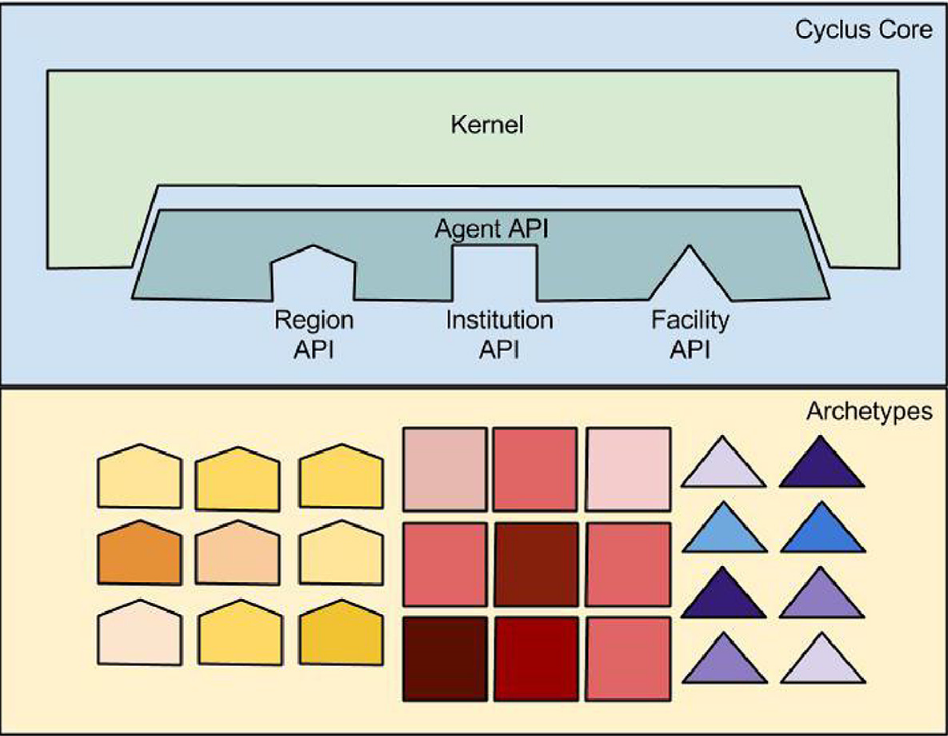
\includegraphics[width=.6\textwidth]{./images/cyclus_structure.png}
        \end{center}
        \caption{Modular Design of Cyclus}
        \label{fig:cyclus_struc}

	\end{figure}
\end{frame}

\begin{frame}
    \frametitle{Timestep Execution}
    A simplified explanation: Each timestep:
    
\begin{figure}[H]
\centering
\scalebox{0.7}{
\begin{tikzpicture}[node distance=1.5cm]
\node (Build) [process] {Build (kernel)};
\node (Tick) [process, below of=Build] {Tick (agent)};
\node (DRE) [process, below of=Tick]{Dynamic Resource Exchange (kernel) };
\node (Tock) [process, below of=DRE]{Tock (agent)};
\node (Decom) [process, below of=Tock] {Decommission (kernel)};
\node (Decision) [process, below of=Decom] {\footnotemark Decision (agent)};

\draw [arrow] (Build) -- (Tick); 
\draw [arrow] (Tick) -- (DRE);
\draw [arrow] (DRE) -- (Tock);
\draw [arrow] (Tock) -- (Decom);
\draw [arrow] (Decom) -- (Decision);
\end{tikzpicture}
}
\end{figure}

\footnotetext{Decision phase is planned to be added in the next release.}
\end{frame}

\begin{frame}
	\frametitle{General Info}
	\begin{itemize}
		\item Written in: C++, Python
		\item Input file: xml, json, python
		\item Output file: .sqlite, .hdf5
	\end{itemize}
\end{frame}


\begin{frame}
	\frametitle{Terminology}
	\begin{itemize}
		\item \textbf{Archetypes}: A collection of logic and behavior which can be configured into a prototype which can then be instantiated in simulation as a agent. Archetypes are represented as C++ classes that inherit from the base cyclus::Agent class. (e.g. Reactor module, Sink module)
		\item \textbf{Prototypes}: Archetype + parameters (e.g. Reactor with input-defined  \texttt{name, cycle time, assembly size, core size etc})
		\item \textbf{Agents}: Every single `entity' in play during simulation (Region, Institution, Facility)
	\end{itemize}
\end{frame}

\begin{frame}
	\frametitle{Terminology}
	\begin{itemize}
		\item \textbf{Region}: The group agent that is a collection of institutions (Can manage / control regions)
		\item \textbf{Institution}: Agent that manages facilities (Can deploy, decommission facilities)
		\item \textbf{Facility}: The agent that `trades' and does calculations (Trades material and transmutes, separates)
	\end{itemize}
\end{frame}

\begin{frame}
	\frametitle{Extensions - Archetypes}
	Since Cyclus is an extensible framework, anyone can develop a new archetype and plug-and-play. (\textcolor{blue}{Institution}, \textcolor{red}{region}, facility otherwise.)
	\begin{itemize}
		\item Cycamore: Sink, Storage, Recipe Reactor, Fuelfab, Enrichment, Source, \textcolor{blue}{DeployInst}, Mixer, Separations, \textcolor{red}{GrowthRegion}
		\item \textcolor{blue}{$^*$D3ploy}: Demand-driven deployment Institution (NEUP 16-10512) 
		\item $^*$CYBORG: Reactor depletion analysis tool using ORIGEN
		\item $^*$CYDER: A CYclus Disposal Environment and Repository object.
		\item $^*$CORRM: Continuous On-line Reprocessing Reactor Module.
		\item $^*$Pyre: Pyroprocessing module with non-proliferation metrics
        \item $^*$Peddler: Simulate trucks and transport material between facilities.
		\item And more..
	\end{itemize}

    \blfootnote{$^*$ Third party module in active development.}
\end{frame}

\begin{frame}
	\frametitle{Extensions - Analysis / Drivers}
	There are other tools to help visualization / output data analysis of Cyclus.
	\begin{itemize}
		\item RICKSHAW: Automated stochastic driver for Cyclus
		\item Cymetric: Extracts important fuel cycle metrics
		\item Analysis: Collection of functions to extract metrics (e.g. natU usage, trade between two facilities, etc.)
		\item Cycmap: GIS visualization tool for Cyclus
		\item Cyclist: GUI for Cyclus (DEPRACATED)
	\end{itemize}
\end{frame}


\begin{frame}
	\frametitle{Installation - Binary}
	Better, more thorough explanations are in \texttt{fuelcycle.org}
	\begin{itemize}
		\item Windows: N/A
		\item MacOS: \texttt{conda install -c conda-forge cyclus cycamore}
		\item Linux: \texttt{conda install cyclus cycamore}
	\end{itemize}
\end{frame}


\begin{frame}
	\frametitle{Installation - Build from Source}
    All source files are open-source, and available on Github.

	\texttt{github.com/cyclus/cyclus} and \texttt{github.com/cycamore/cycamore} has the source files, and guides
	\begin{enumerate}
		\item Clone repository (\texttt{git clone [url]})
		\item Install dependency (see github guide README)
		\item \texttt{python install.py}
	\end{enumerate}
\end{frame}


\begin{frame}
	\frametitle{Installation - TroubleShooting}
	Look for your error message or make a new post in the following Cyclus communities:
	\begin{enumerate}
		\item Github Issue in \texttt{github.com/cyclus/cyclus}
		\item Cyclus google user group
        \item Email jbae11@illinois.edu (me)
	\end{enumerate}
\end{frame}

